\section{Конструкторская часть}

В данном разделе будут рассмотрены схемы алгоритмов обновления гипертекстового документа с использованием DOM, VDOM и алгоритма согласования. 
Также будут найдены их трудоёмкости и произведено их сравнение на основе полученных результатов.

\subsection{Разработка алгоритмов}

На рисунках \ref{fig:dom-algorithm}--\ref{fig:child-reconciliation-algorithm}, представлены схемы алгоритмов обновления документа с использованием DOM, VDOM, а также алгоритма согласования соответственно, разработанных на основании приведённых в части \ref{analysis} описаниях.

\clearpage

\begin{figure}[h]
	\centering
	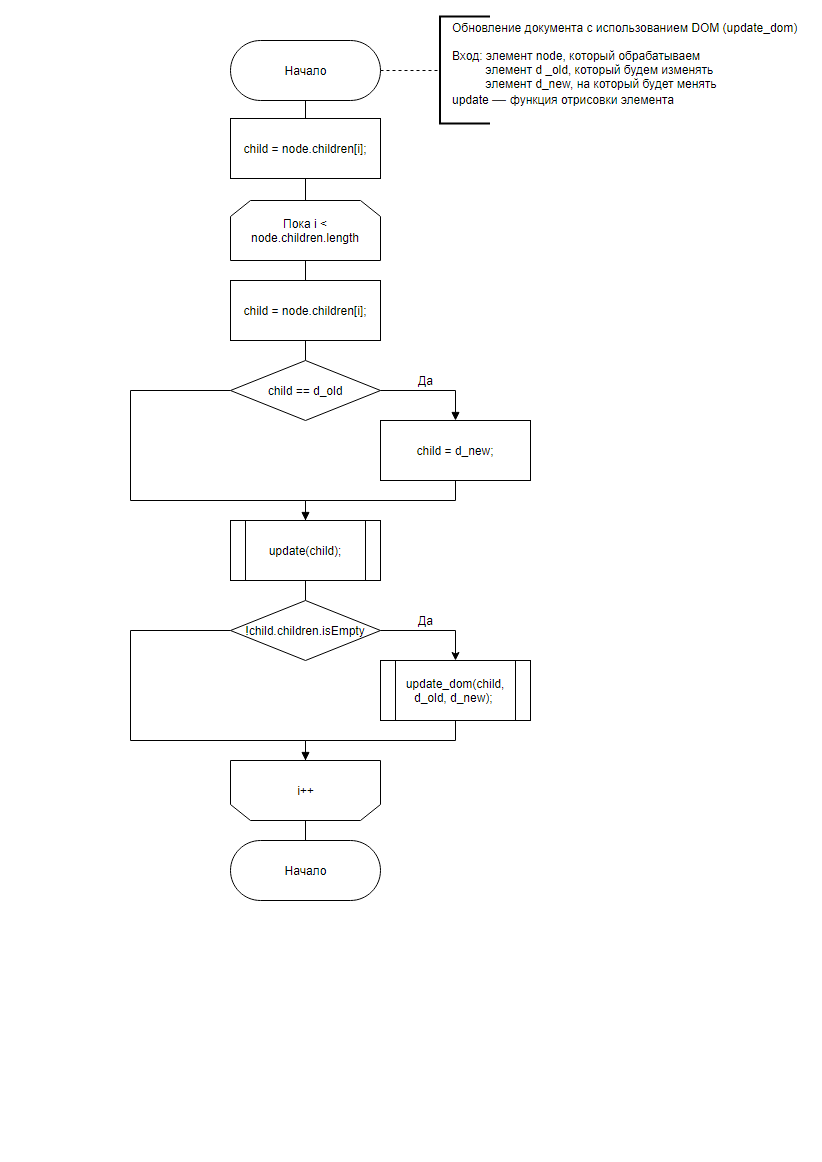
\includegraphics[width=160mm]{img/dom-algorithm.png}
	\caption{Схема алгоритма обновления документа с использованием DOM}
	\label{fig:dom-algorithm}
\end{figure}

\begin{figure}[h]
	\centering
	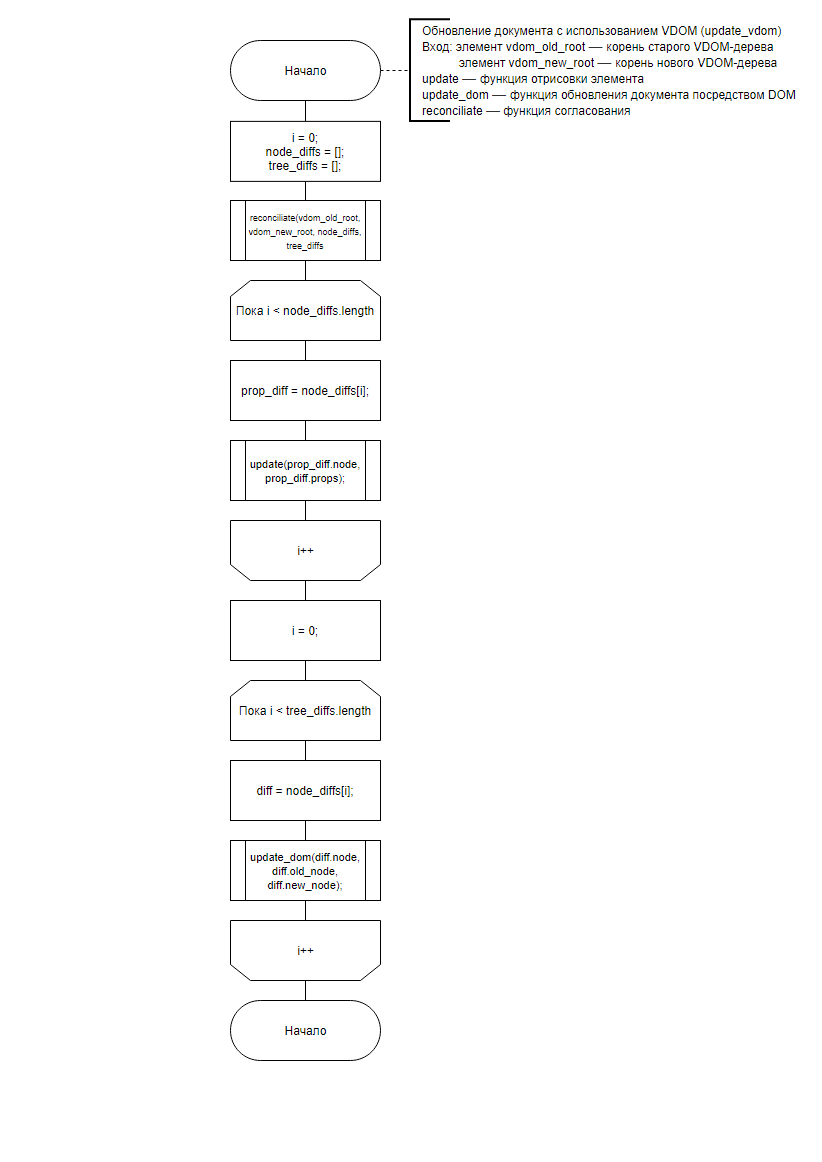
\includegraphics[width=160mm]{img/vdom-algorithm.png}
	\caption{Схема алгоритма обновления документа с использованием VDOM}
	\label{fig:vdom-algorithm}
\end{figure}

\begin{figure}[h]
	\centering
	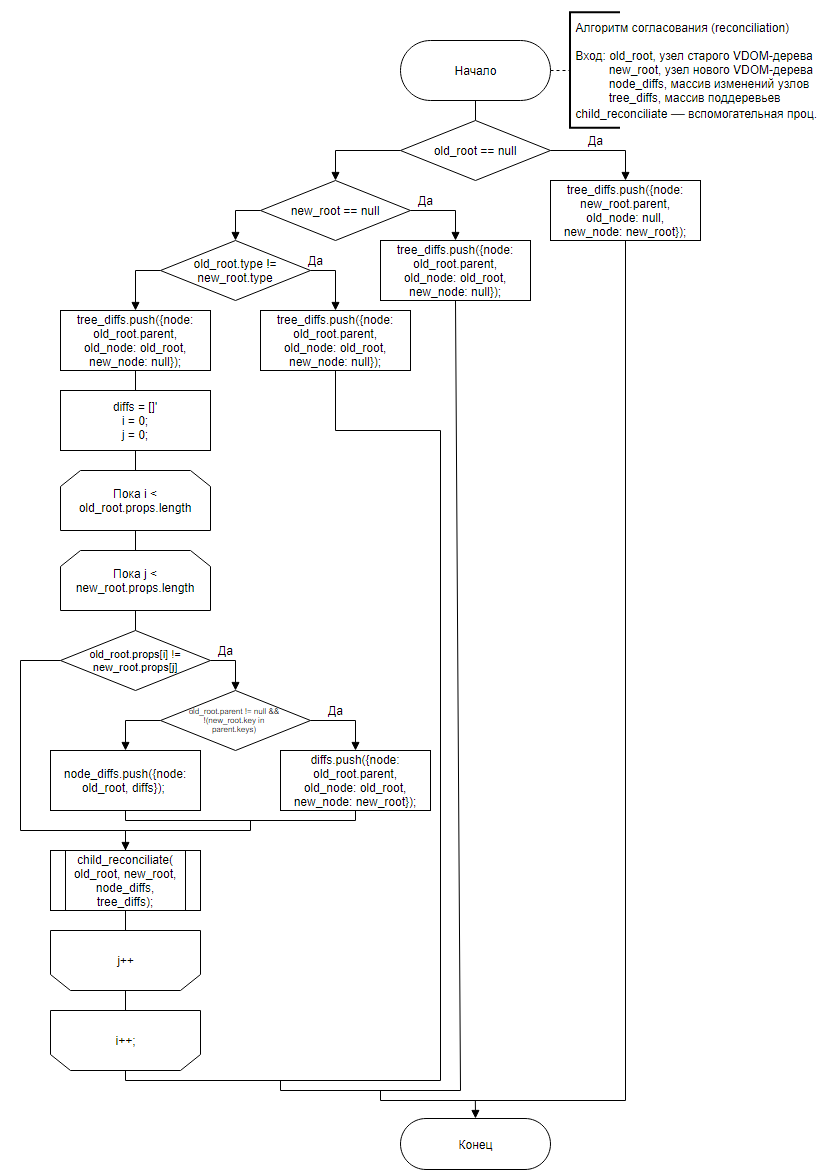
\includegraphics[width=160mm]{img/reconciliation-algorithm.png}
	\caption{Схема алгоритма обновления документа с использованием DOM}
	\label{fig:reconciliation-algorithm}
\end{figure}

\begin{figure}[h]
	\centering
	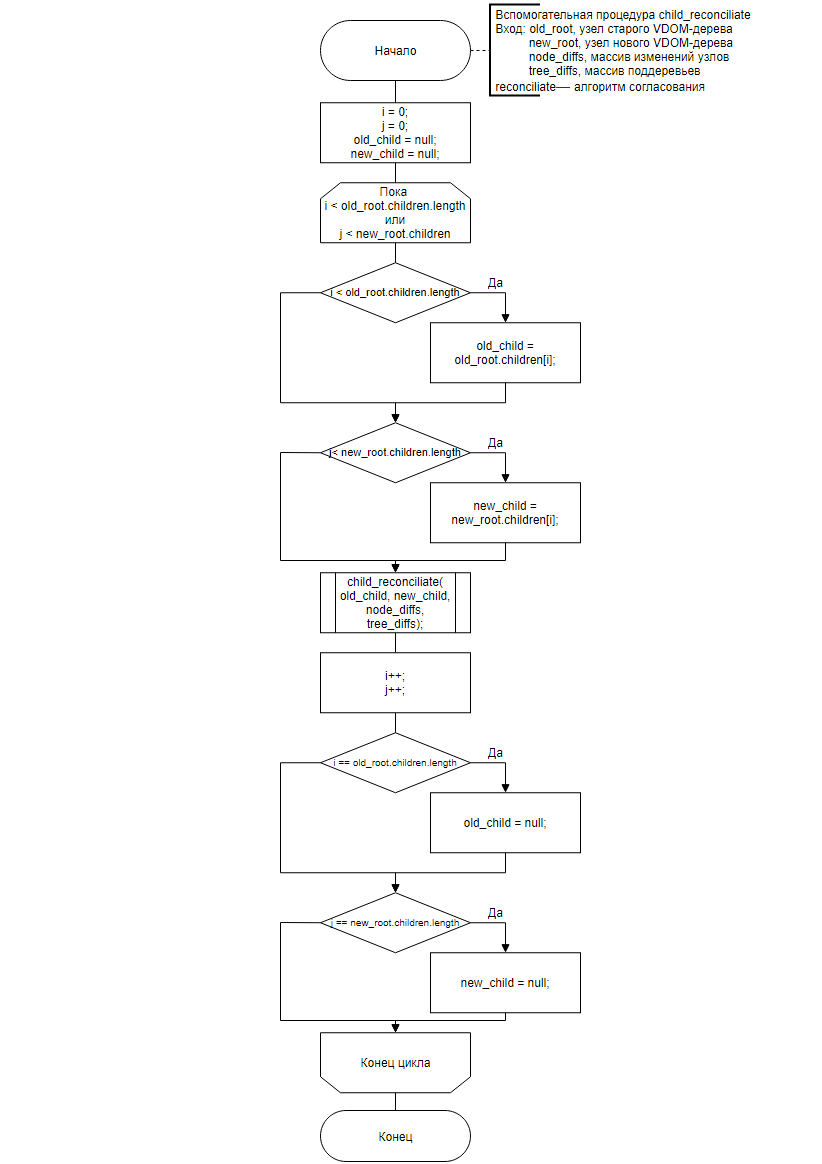
\includegraphics[width=160mm]{img/child-reconciliation-algorithm.png}
	\caption{Схема алгоритма обновления документа с использованием DOM}
	\label{fig:child-reconciliation-algorithm}
\end{figure}

\clearpage

\subsection{Модель вычислений для проведения оценки трудоёмкости}

Введем модель вычислений \cite{model}, которая потребуется для определния трудоемкости каждого отдельно взятого алгоритма сортировки.

\begin{enumerate}[label=\arabic*)]
	\item Операции из списка (\ref{for:operations}) имеют трудоёмкость, равную 1.
	\begin{equation}
		\label{for:operations}
		+, -, /, *, \%, =, +=, -=, *=, ==, !=, <, >, <=, >=, [], ++, {-}-, . 
	\end{equation}
	\item Трудоёмкость оператора выбора \codeword{if условие then A else B} рассчитывается по формуле \ref{for:if}.
	\begin{equation}
		\label{for:if}
		f_{if} = f_{\text{условия}} +
		\begin{cases}
			f_A, & \text{если условие выполняется,}\\
			f_B, & \text{иначе.}
		\end{cases}
	\end{equation}
	\item Трудоёмкость цикла рассчитывается по формуле \ref{for:cycle}.
	\begin{equation}
		\label{for:cycle}
		f_{for} = f_{\text{инициализации}} + f_{\text{сравнения}} + N(f_{\text{тела}} + f_{\text{инкремент}} + f_{\text{сравнения}}).
	\end{equation}
	\item Трудоёмкость вызова функции равна 0.
\end{enumerate}


\subsection{Трудоёмкость алгоритмов}

Определим трудоёмкость выбранных алгоритмов по схемам алгоритмов.

\subsubsection{Алгоритм обновления документа с использованием DOM}

Введём следующие обозначения:
\begin{enumerate}[label=\arabic*)]
	\item $n$ --- количество узлов в DOM-дереве;
	\item $old$ --- случайная величина, значение которой может быть 1 или 0 в зависимсти от того, нужно ли менять значение узла на новое;
	\item $E(old)$ --- математическое ожидание случайной величины $old$;
	\item $x$ --- трудоёмкость операции \codeword{update}, $x >> 1$.
\end{enumerate}

Поскольку величина $old$ может принимать значение 1 только в случае одного узла и 0 во всех остальных случаях, можно найти значение её математического ожидания по формуле \ref{for:e-old}.
\begin{equation}
	\label{for:e-old}
	E(old) = 1 \cdot \frac{1}{n} + 0 \cdot \frac{n - 1}{n} = \frac{1}{n}
\end{equation}

Трудоёмкость алгоритма обновления документа с использованием DOM будет вычисляться по формуле \ref{for:f-dom-1}.
\begin{equation}
	\label{for:f-dom-1}
	f_{dom} = n \cdot (2 + 1 + E(old) + x + 2 + 3)
\end{equation}

C учётом формулы (\ref{for:e-old}) получим итоговую формулу \ref{for:f-dom-2} для расчёта трудоёмкости алгоритма обновления документа с использованием DOM.
\begin{equation}
	\label{for:f-dom-2}
	f_{dom} = xn + 8n + 1
\end{equation}

Поскольку $x >> 1$, $f_{dom} \approx \Theta(xn)$.

\subsubsection{Алгоритм обновления документа с использованием VDOM}
Введём следующие обозначения:
\begin{enumerate}[label=\arabic*)]
	\item $n$ --- количество узлов в изменяемом VDOM-дереве;
	\item $k$ --- случайная величина, которая может принимать значения от 0 до $n$ включительно в зависимсти от того, в каком количестве узлов необходимо изменить содержимое;
	\item $E(k)$ --- математическое ожидание случайной величины $k$;
	\item $t$ --- случайная величина, которая может принимать значения от 0 до $n - k$ включительно в зависимсти от того, какое количество поддеревьев требует полной перерисовки;
	\item $E(t)$ --- математическое ожидание случайной величины $t$;
	\item $x$ --- трудоёмкость операции \codeword{update}, $x >> 1$;
	\item $f_{reconciliate}$ --- трудоёмкость алгоритма согласования.
\end{enumerate}

Поскольку случайная величина $k$ принимает свои значения равновероятно, можно найти её математическое ожидание по формуле \ref{for:e-k}.
\begin{align}
	\begin{split}
		\label{for:e-k}
		E(k) &= \frac{n}{n + 1} + \frac{n - 1}{n + 1}  + \dotsc + \frac{1}{n + 1} + \frac{0}{n + 1} \\
		&= \frac{1}{n + 1} \cdot \frac{(n + 0)\cdot(n + 1)}{2} = \frac{n}{2}
	\end{split}
\end{align}

Аналогичным образом найдём математическое ожидание случайной величины $t$ (формула \ref{for:e-t}).

\begin{align}
	\begin{split}
		\label{for:e-t}
		E(t) &= \frac{n - E(k)}{n - E(k) + 1} + \frac{n - E(k) - 1}{n - E(k) + 1} + \dotsc +  \frac{1}{n - E(k) + 1} \\
		&+\frac{0}{n - E(k) + 1} = \frac{1}{n - E(k) + 1} \cdot \frac{(n - E(k) + 0)\cdot(n - E(k) + 1)}{2}\\
		&= \frac{n - E(k)}{2} = \frac{n}{4}
	\end{split}
\end{align}

Трудоёмкость алгоритма обновления документа с использованием VDOM будет вычисляться по формуле \ref{for:f-dom-1}.
\begin{align}
	\begin{split}
	\label{for:f-vdom-1}
	f_{vdom} &= 2 + f_{reconciliate} + 2 + E(k)\cdot(3 + x) + 2 + E(t)\cdot(3 + f_{dom}) \\
	&= E(k) \cdot (x + 3) + E(t) \cdot (f_{dom} + 3) + 6
	\end{split}
\end{align}

С использованием формул (\ref{for:e-k}) и (\ref{for:e-t}) получим итоговую формулу \ref{for:f-vdom-2} расчёта трудоёмкости алгоритма обновления документа с использованием VDOM.
\begin{equation}
	\label{for:f-vdom-2}
	f_{vdom} = \frac{n \cdot (3 + x)}{2} + \frac{n\cdot(3 + f_{dom})}{2} + f_{reconciliate} + 6
\end{equation}


\subsubsection{Алгоритм согласования}

Для алгоритма согласования рассмотрим худший и лудший случай.

Худшим случаем будем считать случай, при котором необходимо изменить все параметры всех узлов дерева, и добавить новые узлы в каждый из листовых узлов.
Введём следующие обозначения:
\begin{enumerate}[label=\arabic*)]
	\item $n$ --- количество узлов в изменяемом VDOM-дереве;
	\item $m$ --- количество параметров в одном узле;
	\item $k$ --- количество узлов изменяемого VDOM-дерева;
	\item $\lambda$ --- количество новых узлов, добавлемых в каждый лист изменяемого VDOM-дерева.
\end{enumerate}

Тогда трудоёмкость алгоритма согласования для худшего случая может быть вычислена по формуле \ref{for:f-reconciliation-worst}.

\begin{align}
	\begin{split}
		\label{for:f-reconciliation-worst}
		f_{reconciliate_{worst}} &= (n + \lambda) \cdot (5 + 1 + 2 + m \cdot (3 + 2 + m \cdot (3 + 1 + 3)) \\
		&+ 2 + 7 + 4 + 4 + 7) + (n + \lambda) \cdot (2 + 2 + 2) + n \cdot 3 \\
		&+ (n + \lambda) \cdot 3 + \lambda + 1 =\\
		&= (n + \lambda) \cdot (41 + m \cdot (5 + 7m)) + 3n + \lambda + 1 \\
		&= (7m^2 + 5m)\cdot(n + \lambda) + 44n + 42\lambda + 1
	\end{split}
\end{align}

Лучшим случаем для алгоритма согласования будем считать случай, при котором разница в типе узла находится в первом же узле, т.е. возникает необходимость перерисовать всё дерево целиком, что является худшим случаем для алгоритма обновления документа с использованием VDOM и алгоритма согласования.

Трудоёмкость алгоритма согласования для лучшего случая считается по формуле \ref{for:f-reconciliation-best}.

\begin{align}
	\begin{split}
		\label{for:f-reconciliation-best}
		f_{reconciliate_{best}} &= 1 + 2 + 2 + 4 = 9
	\end{split}
\end{align}

\subsection{Сравнение трудоёмкостей алгоритмов}

Сравним трудоёмкости алгоритмов обновления документа с использованием DOM и VDOM.

Трудоёмкость алгоритма обновления документа с использованием DOM была вычислена по формуле (\ref{for:f-dom-2}) и не зависит только от двух параметров, являясь пропорциональной $\Theta(xn)$, где $x$ --- трудоёмкость операции update отрисовки узла, а $n$ --- количество узлов в новом DOM-дереве.

Трудоёмкость алгоритма обновления документа с использованием VDOM и алгоритма согласования зависит от того, насколько предположения, заложенные в основу эвристики алгоритма согласования, выполняются.

Так, если процесс изменения производится с учётом данных предположений, будет некорректно считать результат работы алгоритма согласования равновероятным, и, следовательно, считать трудоёмкость использующего его алгоритма обновления посредством VDOM через формулу (\ref{for:f-vdom-2}). 
Однако трудоёмкость, вычисленная посредством формулы (\ref{for:f-vdom-1}) остаётся верной, поэтому дальнейшие выводы будут сделаны, основываясь на данной формуле.

Чем лучше соблюдаются предположения, положенные в основу алгоритма согласования, чем меньше будет величина $t$, т.е. количество поддеревьев, требующиъ полной перерисовки. 
То есть трудоёмкость алгоритма будет пропорциональна $\Theta(xk)$, где $k$ --- количество узлов, требующих перерисовки, $k << n$ в общем случае.

Иными словами, алгоритм обновления документа с использованием VDOM и алгоритма согласования будет иметь меньшую трудоёмкость, чем алгоритм обновления документа с использованием DOM, за счёт понимания того, какие узлы нужно перерисовывать, а какие нет.

Стоит отметить, что при несоблюдении предположений, на которых основывается алгоритм согласование, трудоёмкость алгоритма с использованием VDOM будет превышать трудоёмкость алгоритма, использующего DOM. 
Такая ситуация произойдёт, например, при постоянном изменении типа корневого элемента.

\subsection*{Вывод}

Были разработаны схемы алгоритмов обновления гипертекстового документа с использованием DOM, VDOM и алгоритма согласования. Были найдены их трудоёмкости и произведено их сравнение.

Трудоёмкость алгоритма обновления документа с использованием DOM пропорциональна $\Theta(xn)$, где $x$ --- трудоёмкость операции update отрисовки узла, а $n$ --- количество узлов в новом DOM-дереве.
В это время трудоёмкость обновления документа с использованием VDOM и алгоритма согласования в случае соблюдения предположений, лежащих в основе алгоритма согласования, пропорциональна $\Theta(xk)$, где $k$ --- количество узлов, требующих перерисовки, $k << n$ в общем случае.

Таким образом, алгоритм обновления гипертекстового документа с использованием VDOM и алгоритма согласования имеет меньшую трудоёмкость при соблюдении эвриситки агоритма согласования, за счёт перерисовки только необходимых улов.
В противном случае, когда эвристика алгоритма согласования не соблюдена, использование VDOM может иметь большую трудоёмкость, чем просто использование DOM.

\pagebreak